\section{Úvod}
Cieľom merania je meranie malých zmien odporu (použitie tenzometra). Meranie je realizované v simulačnom prostredí KiCad. K výpočtu presnosti merania uvažujeme použitie 12-bitového AD prevodníku s rozsahom $0-3,3V$.

Pri použití digitálneho prevodníku je chyba meranej hodnoty rovná polovici najmenšieho rozdielu rôznych výstupných hodnôt. Pre použitý AD prevodník je chyba $ = \frac{3,3}{2^{12}-1}*0,5 \doteq 0,40293$mV. 
% Neistota merania $u_B(U)$ sa teda rovná $u_B(U) = \frac{\frac{3,3}{2^{12}-1}*0,5}{\sqrt{3}} \doteq 0,00023263$V

V kapitole \ref{a} je popísané meranie napäťovým deličom.
V kapitole \ref{b} je popísané meranie s využitím wheatstonovho mostíku.

Schéma meraní z kapitol \ref{a} a \ref{b} je uložená v súbore \texttt{SEM-Proj2-1\_2.kicad\_sch}.

V kapitole \ref{c} je popísané meranie s využitím operačného zosilňovaču a odpovedajúca schéma je uložená v súbore \texttt{SEM-Proj2.kicad\_sch}.

\section{Meranie pomocou napäťového deliča}
\label{a}

Schéma \ref{fig:enter-label} zobrazuje zapojenie napäťového deliča.
K meraniu bol použitý $3,3$V zdroj z dôvodu zhodného rozsahu s použitým AD prevodníkom.
Hodnota odporu $R_1 = 200$ bola zvolená tak, aby bola rovná odporu nezaťaženého tenzometra. 
Hodnota $R$ odporu termistoru je určená vzťahom \ref{v1}:
\begin{equation}
    \label{v1}
    R = \frac{V_1}{\frac{Vcc_1 - V_1}{R_1}}
\end{equation}

Dosiahnuté hodnoty merania odporu a hmotnosti sú zhrnuté v tabuľke \ref{t1}.

%Výsledný odpor je $(R \pm 0,024423)\ohm$.

%Výsledná hmotnosť je $(|M \pm 0.00610575161|)kg$. 

Tenzometer nameral zápornú hmotnosť, fyzikálne ale nie je záporná hmotnosť správne a je nutné použiť absolútnu hodnotu nameraných hodnôt. Záporné hodnoty sú spôsobené použitím tenzometru v závernom smere.
\begin{figure}[H]
    \centering
    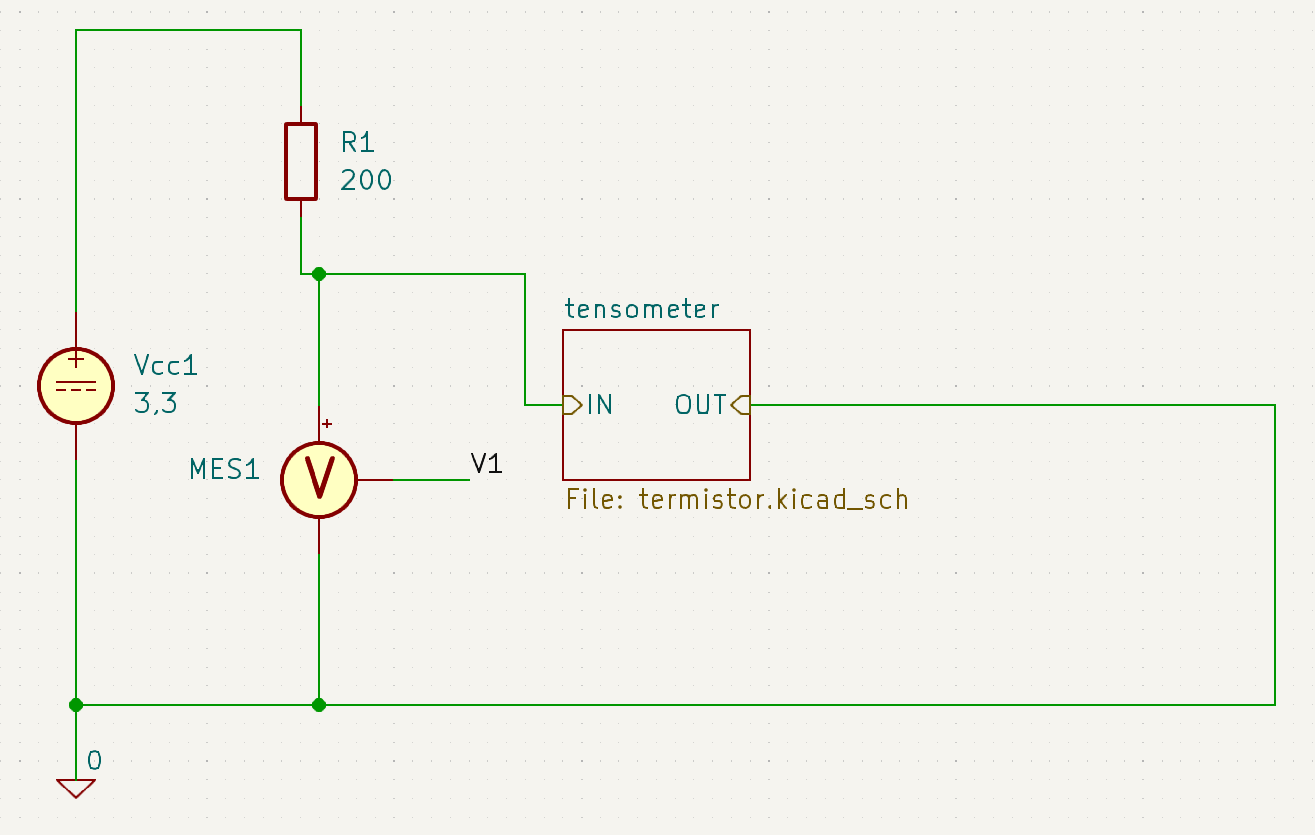
\includegraphics[width=0.7\linewidth]{fig/jedna.png}
    \caption{Schéma zapojenia napäťového deliča}
    \label{fig:enter-label}
\end{figure}
\begin{table}[H]
    \centering
    \begin{tabular}{|r|c|c|c|c|}
        \hline
         $t = 2n , n \in \mathbb{N}$ &  $a$ &  $b$ & R &M\\
        \hline
         1&  t + 0,001&  t + 0,2& 200.187&-0.0467\\
        \hline
         2&  t + 0,23&  t + 0,45&  202.849&-0.7123\\
        \hline
         3&  t + 0,55&  t + 0,70&  202.483&-0.6208\\
        \hline
         4&  t + 0,80&  t + 1,30&  202.768&-0.6920\\
        \hline
         5&  t + 1,35&  t + 1,60&  202.894&-0.7234\\
        \hline
         6&  t + 1,79&  t + 2,00&  201.785&-0.4462\\
        \hline
    \end{tabular}
    \caption{Namerané hodnoty odporu R a hmotnosti M v časových intervaloch $<a,b>$ pomocou napäťového deliča.}
    \label{t1}
\end{table}



\section{Meranie pomocou wheatstonovho mostíku}
\label{b}
Schéma zapojenia mostíku je znázornená na obrázku \ref{fig:2}. Hodnota odporu $R$ sa určuje z hodnôt napájacieho napätia $Vcc_2 = 3,3$, rozdielu napätí $V_2 = V_{11} - V_{22}$ a odporov $R_1 = R_6 = R_5$. Vzťah pre výpočet hodnoty $R$ pomocou wheatstonovho mostíku platí vzťah \ref{v2}. 
\begin{equation}
    \label{v2}
    R = \frac{R_1*Vcc_2-2R_1*V_2}{R_1*Vcc_2+2R_1*V_2}*R_1
\end{equation}
Dosiahnuté výsledky sú zhrnuté v tabuľke \ref{t2}.
\begin{figure}[H]
    \centering
    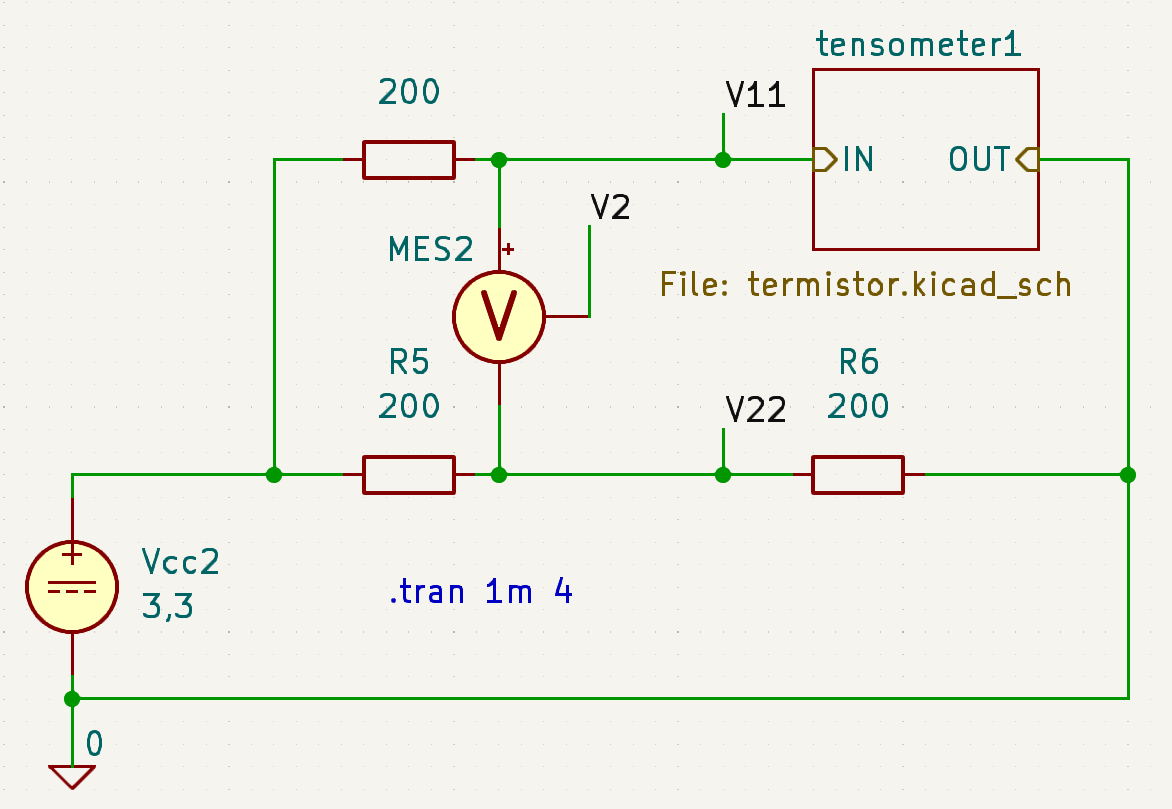
\includegraphics[width=0.7\linewidth]{fig/dva.png}
    \caption{Schéma zapojenia wheatstonovho mostíku}
    \label{fig:2}
\end{figure}
\begin{table}[H]
    \centering
    \begin{tabular}{|r|c|c|c|c|}
        \hline
         $t = 2n , n \in \mathbb{N}$ &  $a$ &  $b$ & R &M\\
        \hline
         1&  t + 0,001&  t + 0,2& 200.188&-0.047\\
        \hline
         2&  t + 0,23&  t + 0,45& 202.848&-0.712\\
        \hline
         3&  t + 0,55&  t + 0,70& 202.483&-0.6208\\
        \hline
         4&  t + 0,80&  t + 1,30& 202.768&-0.6921\\
        \hline
         5&  t + 1,35&  t + 1,60& 202.893&-0.7232\\
        \hline
         6&  t + 1,79&  t + 2,00& 201.784&-0.4459\\
        \hline
    \end{tabular}
    \caption{Namerané hodnoty odporu R a hmotnosti M v časových intervaloch $<a,b>$ pomocou wheatstonovho mostíku.}
    \label{t2}
\end{table}
\section{Meranie pomocou wheatstonovho mostíku s operačným zosilňovačom}
\label{c}
Schéma \ref{fig:3} zobrazuje zapojenie z predchádzajúcej úlohy s využitím operačného zosilňovaču.
Hodnota odporov, ktoré boli pridané oproti zapojeniu zapojeniu v predošlej kapitole, boli experimentálne nastavené na hodnotu $R_f = 20$k$\ohm$. Hodnota odporu $R$ termistoru je určená vzťahom \ref{v3}:
\begin{equation}
    \label{v3}
    R = R_1(1+\frac{2R_1V_3}{R_fUcc_2-R_1V_3})
\end{equation}

Dosiahnuté hodnoty merania odporu a hmotnosti sú zhrnuté v tabuľke \ref{t3}.
\begin{figure}[H]
    \centering
    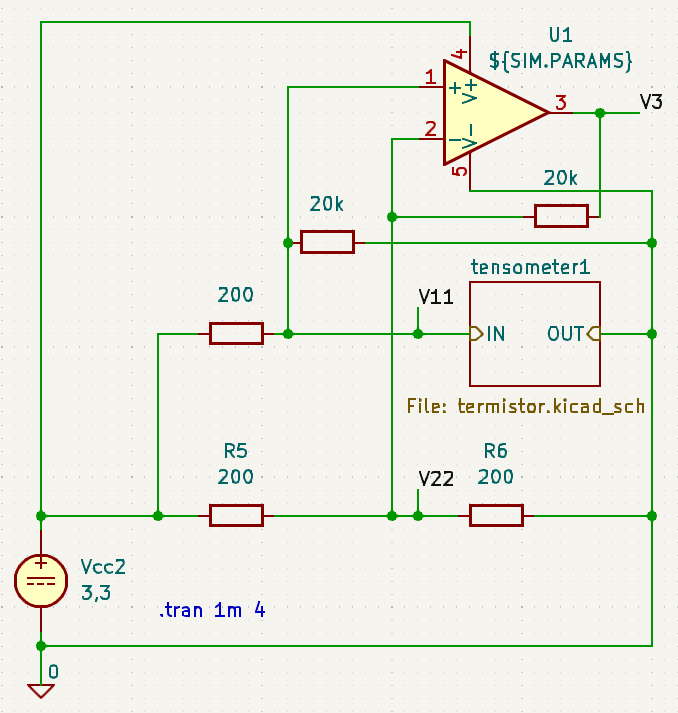
\includegraphics[width=0.5\linewidth]{fig/triS.png}
    \caption{Schéma zapojenia wheatstonovho mostíku s operačným zosilňovačom}
    \label{fig:3}
\end{figure}
\begin{table}[H]
    \centering
    \begin{tabular}{|r|c|c|c|c|}
        \hline
         $t = 2n , n \in \mathbb{N}$ &  $a$ &  $b$ & R &M\\
        \hline
         1&  t + 0,001&  t + 0,2& 201.275&-0.3187\\
        \hline
         2&  t + 0,23&  t + 0,45& 202.721&-0.6802\\
        \hline
         3&  t + 0,55&  t + 0,70& 202.662&-0.6654\\
        \hline
         4&  t + 0,80&  t + 1,30& 202.714&-0.6784\\
        \hline
         5&  t + 1,35&  t + 1,60& 202.724&-0.681\\
        \hline
         6&  t + 1,79&  t + 2,00& 202.021&-0.5054\\
        \hline
    \end{tabular}
    \caption{Namerané hodnoty odporu R a hmotnosti M v časových intervaloch $<a,b>$ pomocou wheatstonovho mostíku s operačným zosilňovačom.}
    \label{t3}
\end{table}
\section{Záver}
Správanie simulovaného tenzometra bolo zmerané tromi metódami. Z namerania negatívnej hmotnosti je zrejmé, že tenzometer bol použitý v opačnom smere, než aký je udávaný štandardne. V prípade prvého, resp. druhého merania bol rozdiel najvyššej a najnižšej nameranej hodnoty na prevodníku 15, resp. 16 jednotiek prevodníku. To je $0,37\%$, resp. $0,39\%$ rozsahu prevodníku. S využitím operačného zosilňovaču bolo medzi najvyššou a nižšou hodnotou až $1470$ hodnôt, teda bolo využitých až $35,89\%$ rozsahu. 
% Presnosť merania so zosilňovačom teda vzrástla až o dva rády. 
Meranie bolo presné.